\documentclass{article}

    % Input language encoding
    \usepackage[utf8]{inputenc}
   
    % Output languages
    \usepackage[english, greek]{babel}
    \usepackage{alphabeta}
    
    % Fonts
    \usepackage[T1,LGR]{fontenc}
    \usepackage{lmodern}

    % Images
    \usepackage{graphicx}
    \usepackage{float}
    \usepackage{caption}
    \usepackage{subcaption}

    % Math
    \usepackage{amsmath}
    \usepackage{amssymb}

    % Paragraph Formatting
    \usepackage{parskip}

    % Code
    \usepackage{listings}
    \usepackage{fancyvrb}

    % Different Enumerations
    \usepackage{enumitem}

    % Trees
    \usepackage{qtree}

    % Other Drawings
    \usepackage{tikz}
    \usetikzlibrary{shapes,backgrounds}

    % Links
    \usepackage{hyperref}

    % Color
    \usepackage{color}
   
    % Setup

    % For hyperlinks
    \hypersetup{
        colorlinks=true,
        linkcolor=blue,
        filecolor=magenta,      
        urlcolor=cyan,
    }

    \urlstyle{same}
    
    % For code
    \definecolor{codegreen}{rgb}{0,0.6,0}
    \definecolor{codegray}{rgb}{0.5,0.5,0.5}
    \definecolor{codepurple}{rgb}{0.58,0,0.82}
    \definecolor{backcolour}{rgb}{0.95,0.95,0.92}
     
    \lstdefinestyle{mystyle}{
        backgroundcolor=\color{backcolour},   
        commentstyle=\color{codegreen},
        keywordstyle=\color{magenta},
        numberstyle=\tiny\color{codegray},
        stringstyle=\color{codepurple},
        basicstyle=\fontsize{8}{11}\selectfont\ttfamily,
        breakatwhitespace=false,         
        breaklines=true,                 
        captionpos=b,                    
        keepspaces=true,                 
        numbers=left,                    
        numbersep=5pt,                  
        showspaces=false,                
        showstringspaces=false,
        showtabs=false,                  
        tabsize=4
    }

    \lstset{style=mystyle}

    % For math
    \DeclareMathSizes{10}{10}{10}{10}
    \setlength{\parindent}{0cm}

    % Foreign Language macro
    \newcommand{\english}[1]{\foreignlanguage{english}{{#1}}}

    \title{1η Εργαστηριακή Ασκήσεων \\
        Σχεδιασμός Ενσωματωμένων Συστημάτων}
\begin{document}

\pagenumbering{arabic}
\date{}
\author{Λεωνίδας Αβδελάς $|$ ΑΜ: 03113182}

\maketitle
\newpage

\section*{Ζητούμενο 1ο - \english{Loop Optimizations \\ \& Design Space Exploration}}

\subsection*{1.}
\begin{itemize}
    \item Για την έκδοση λειτουργικού και την έκδοση πυρήνα \english{Linux}, θα χρησιμοποιήσουμε τις εντολές \english{\lstinline[language=bash]{cat /etc/os-release}} και \english{\lstinline[language=bash]{uname -r}}, αντίστοιχα. Τα αποτελέσματα είναι \english{PRETTY\_NAME=Debian GNU/Linux 10 (buster)} και \english{4.19.0-6-amd64}.
    \item Για την ιεραρχία μνήμης, χρησιμοποιήσαμε την εντολή \english{\lstinline[language=bash]{sudo lshw -C memory}}. Τα αποτελέσματα φαίνονται στον παρακάτω πίνακα:\\
    \begin{otherlanguage}{english}
        \begin{center}
            \begin{tabular}{|c|c|c|c|c|}\hline
                & L1 cache & L2 cache & L3 cache & RAM \\ \hline
                Size & 32KiB & 256KiB & 3MiB & 8GiB \\ \hline
           \end{tabular}
        \end{center}
        \end{otherlanguage}
    \item Τις πληροφορίες για τους πυρήνες θα τις βρούμε στο αρχείο \english{/proc/cpuinfo}. Έτσι, για τον αριθμό των πυρήνων, τρέχουμε:
    \\ \english{\lstinline[language=bash]{cat /proc/cpuinfo \| grep processor \| wc -l}} \\
    από όπου παίρνουμε την απάντηση 4 και για την ταχύτητα τους, τρέχουμε :\\
    \english{\lstinline[language=bash]{cat /proc/cpuinfo \|  grep 'cpu MHz'}} \\
    από όπου παίρνουμε την απάντηση \english{~800Mhz}.
\end{itemize}

\subsection*{2.}

Προσθέτοντας τον υπολογισμό χρόνου στο πρόγραμμα μας και τρέχοντας το 10 φορές, έχουμε τα παρακάτω αποτελέσματα: \\
\begin{otherlanguage}{english}
    \begin{center}
        \begin{tabular}{|c|c|c|c|}\hline
            & Average & Maximum & Minimum \\ \hline
            Time &  11796.1us & 15874us & 11335ms\\ \hline
       \end{tabular}
    \end{center}
    \end{otherlanguage}

    Ένα πράγμα που παρατηρούμε ότι η διαδοχικές εκτελέσεις του προγράμματος επωφελούνται από το \english{caching} των δεδομένων. Έτσι, η πρώτη φορά που τρέχει το πρόγραμμα απαιτεί τον μέγιστο χρόνο, και οι επόμενες απαιτούν αισθητά λιγότερο χρόνο. 

\subsection*{3.}

Εξατάζουμε τον κώδικα, η πρώτη αλλαγή που βλέπουμε ότι μπορεί να γίνει είναι ένα \english{loop merging} των loops για τον άξονα x. Έτσι γλυτώνουμε \english{B} επαναλήψεις για κάθε \english{pixel}.

Μετά από μελέτη των μετασχηματισμών, δεν μπορέσαμε να βρούμε κάποιον άλλο που θα μπορούσε να μειώσει την ταχύτητα του προγράμματος και να μπορεί να γίνει χειροκίνητα. Τα αποτελέσματα μας για αυτό το βήμα είναι:

\begin{otherlanguage}{english}
    \begin{center}
        \begin{tabular}{|c|c|c|c|}\hline
            & Average & Maximum & Minimum \\ \hline
            Time &  10975.us & 15245us & 10475ms\\ \hline
       \end{tabular}
    \end{center}
    \end{otherlanguage}

Όπως είναι εύκολο να δούμε, υπάρχει μια μεγάλη μείωση στον χρόνο εκτέλεσης του προγράμματος μας, αφού η ταχύτητα μειώθηκε κατα σχεδόνο \english{$1000us$}, δηλαδή \english{$1ms$}.

\subsection*{4.}

Χρησιμοποιώντας \english{DSE}, για το μέγεθος του \english{B} για τιμές που είναι κοινοί διαιρέτες του M και του Ν, βλέπουμε ότι το βέλτιστο μέσο χρόνο τον έχουμε για $B = 16$, με μέση τιμή $9532.4$.

Δεν υπάρχει κάποια ακριβής συσχέτιση μεταξύ των δεδομένων του ερωτήματος 1 και των αποτελεσμάτων εδώ. Εφ'όσον το \english{$B$} είναι δύναμη του $2$ και οι \english{caches} του υπολογιστή επίσης είναι δύναμη του $2$ και πολλαπλάσιο του $16$, το μεγαλύτερο μέγεθος \english{$B$} εξασφαλίζει μικρότερο αριθμό επαναλήψεων στ εξωτερικό \english{loop}.

\subsection*{5.}
Το ζεύγος \english{$B_x$} και \english{$B_y$} για το οποίο πετυχαίνουμε την καλύτερη απόδοση είναι το $(144, 176)$ με μέσο χρόνο \english{$9858.22us$}.
Για να περιορίσουμε την αναζήτηση σε μικρότερο αριθμό παραμέτρων, θα μπορούσαμε πρώτα από όλα να δοκιμάσουμε για τιμές μεγαλύτερες του 16 τόσο για το \english{$B_x$} όσο και για το \english{$B_y$}, αφού στο προηγούμενο ερώτημα ήδη έχουμε βρει ότι η καλύτερη απόδοση για τετράγωνο Β είναι το 16. Έτσι θα αποφεύγαμε αρκeτές επαναλήψεις στις χαμηλότερες τιμές.

\subsection*{6.}
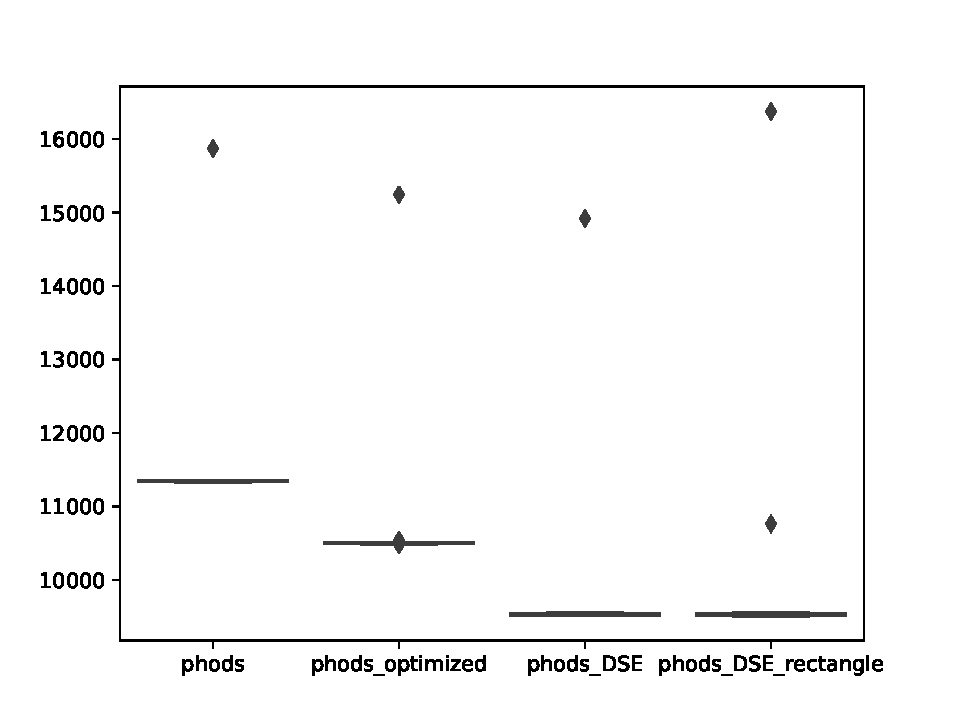
\includegraphics[scale=0.65]{Part1/results/results_boxplots.pdf}

Παρατηρούμε ότι όλα τα προγράμματα έχουν ένα τρέξιμο με πολύ μεγάλο χρόνο σχετικά με τον μέσο όρο. Αυτό συμβαίνει γιατί στα διαδοχικά τρεξίματα έχουμε επαναχρησιμοποίηση των δεδομένων στην cache και έτσι μειωμένους χρόνος. Ακόμα, η βελτίωση μεταξύ του βήματος 4 και βήματος 5 είναι πολύ μικρή, και αρα η μεγαλύτερη αναζήτηση δεν είναι απαραίτητα χρήσιμη. Αυτό συμβαίνει γιατί μετά από κάποιο σημείο (και επειδή ο υπολογιστής που χρησιμοποιήσαμε είναι αρκετά σύγχρονος και γενικού σκοπού), οι καθυστερήσεις οφείλονται σε άλλους παράγοντες και όχι στο ίδιο το πρόγραμμα.
\end{document}